\section{Differential geometry}
\label{section: differential geometry}


General relativity, and a lot of quantum field theory, are formulated in the language of \emph{differential geometry}.
Differential geometry generalizes $n$-dimensional calculus to more general spaces than the usual $\R^n$, such as curved spacetime or the more abstract space of symmetries of a quantum field theory.
This section is based on~\autocite{carrollSpacetimeGeometryIntroduction2019,leeIntroductionSmoothManifolds2003d}.

\begin{figure}[H]
    \centering
    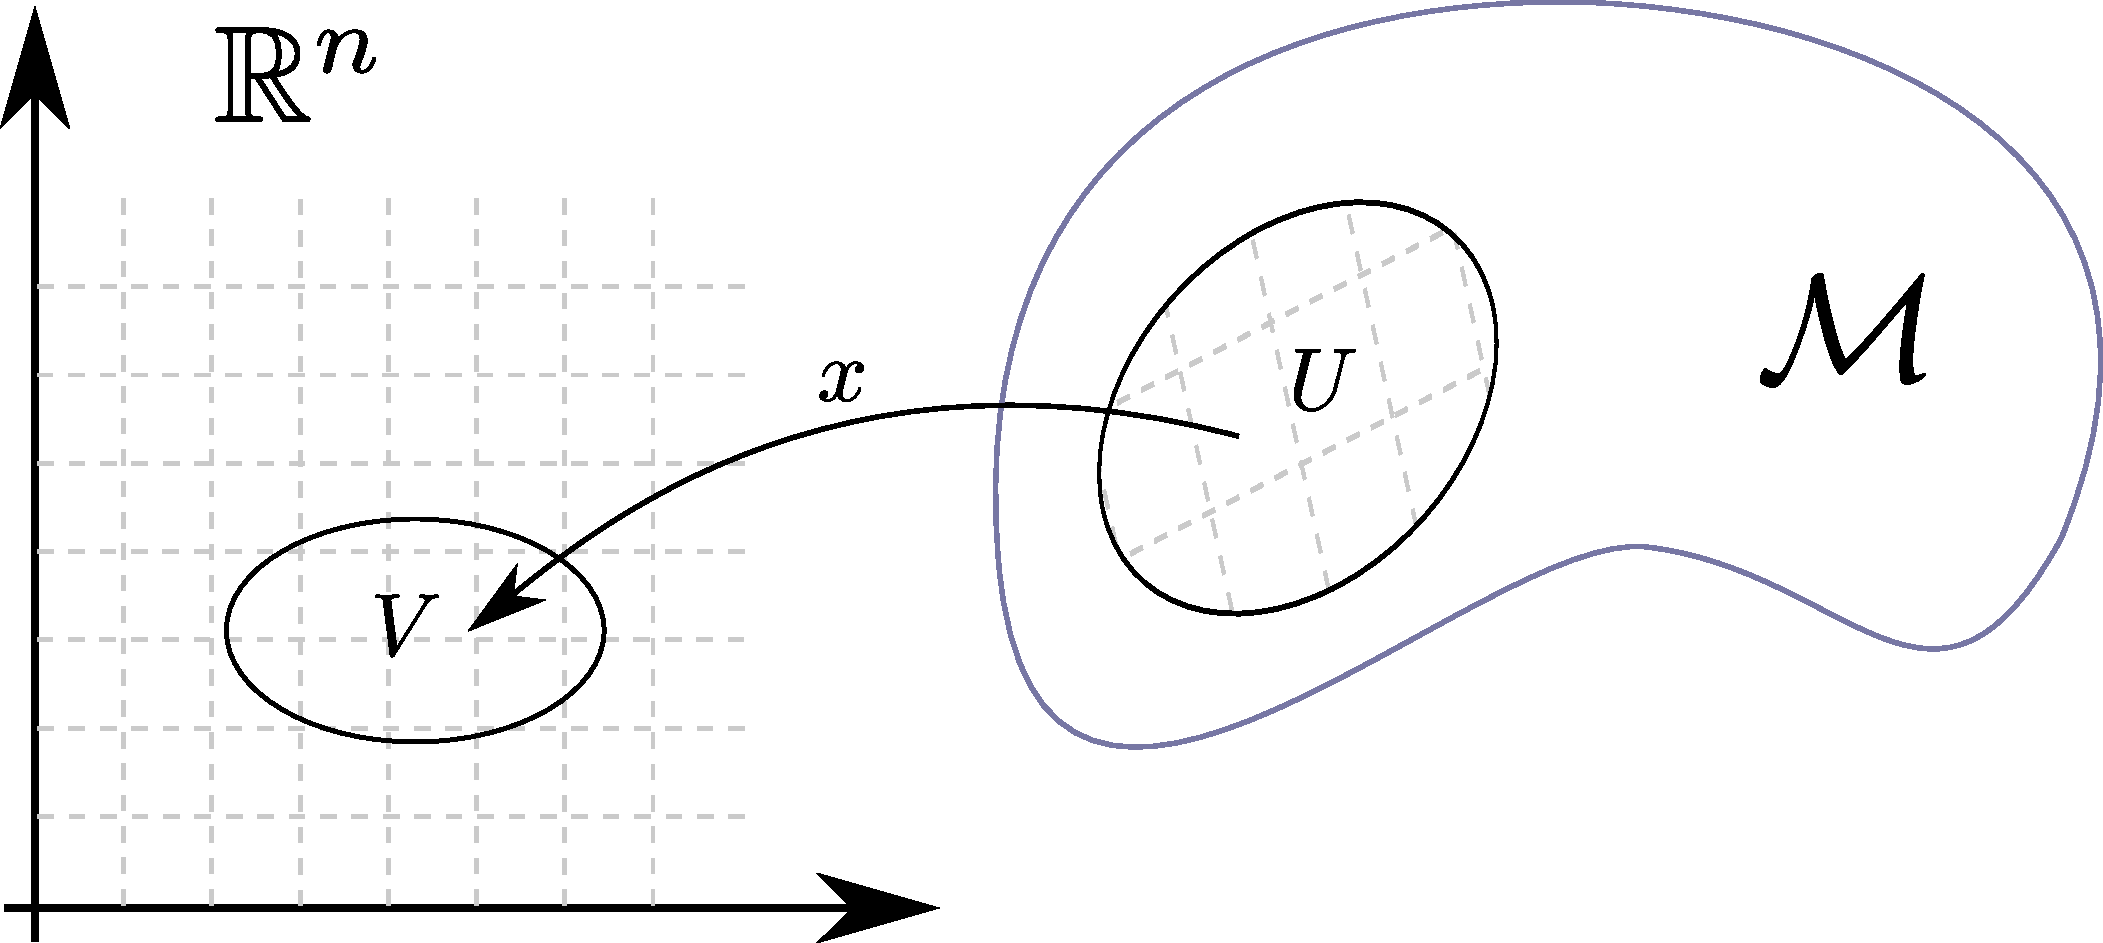
\includegraphics[width=0.7\textwidth]{figurer/coordinate_function.pdf}
    \caption{
        The coordinate function $x$ maps a neighborhood $U$ in the manifold $\Em$ to a neighborhood $V$ in $\R^n$.
        }
    \label{fig: coordinate function}
\end{figure}



\subsection{Manifolds and coordinates}


The most important objects in differential geometry are \emph{smooth manifolds}.
An $n$-dimensional manifold, $\Em$, is a set of points, locally homeomorphic to $\R^n$.
That is, for all points $p \in \Em$, there exists a neighborhood $U$ around $p$, together with a corresponding set of continuous, bijective functions that map $U$ to a neighborhood $V$ in $\R^n$,
%
\begin{align}
    x: U \subseteq \Em & \longmapsto V \subseteq \R^n, \\
    p & \longmapsto x^\mu(p), \quad \mu \in \{0, \dots, n-1\}.
\end{align}
%
This is illustrated in \autoref{fig: coordinate function}.
We call $x(p) = (x^0(p), \dots, x^{n- 1}(p))$ a coordinate function of $\Em$.
The inverse of $x$, $x^{-1}$, obeys $x^{-1}(x(p)) = p$, for all $p \in U$.
A smooth manifold is one in which the coordinate functions are infinitely differentiable.
To define differentiability on manifolds, consider two coordinate functions, $x$, and $x'$.
The corresponding domains $U$ and $U'$ may or may not overlap.
We then define the transition function, a function between subsets of $\R^n$ by mapping via $\Em$, as
%
\begin{align}
    f_{x\rightarrow x'} = x \circ {x'}^{-1} : \R^n \mapsto \R^n.
\end{align}
%
This map is illustrated in \autoref{fig: transition map}.\footnote{
    To be rigorous, one has to restrict the domains and image of the coordinate function when combining them. This is illustrated in \autoref{fig: transition map}.
    }
A set of coordinate functions $\mathcal A = \{x_i\}$ whose domain cover $\Em$ is called an \emph{atlas} of $\Em$.
If the transition function between all pairings of coordinate functions in the atlas is smooth---that is, infinitely differentiable---we call the atlas smooth.
We then define a smooth manifold as the topological manifold $\Em$ together with a \emph{maximal} smooth atlas $\mathcal A$.
A smooth atlas is maximal if no coordinate function can be added while the atlas remains smooth.\footnote{
    The maximal condition ensures that two equivalent atlases correspond to the same differentiable manifold. A single manifold can be combined with different maximal atlases of smooth coordinates or differentiable structures. A set of examples are \emph{exotic spheres}, smooth manifolds which are \emph{homeomorphic} to $\text S^n$, but not \emph{diffeomorphic}. 
    }
%
\begin{figure}[H]
    \centering
    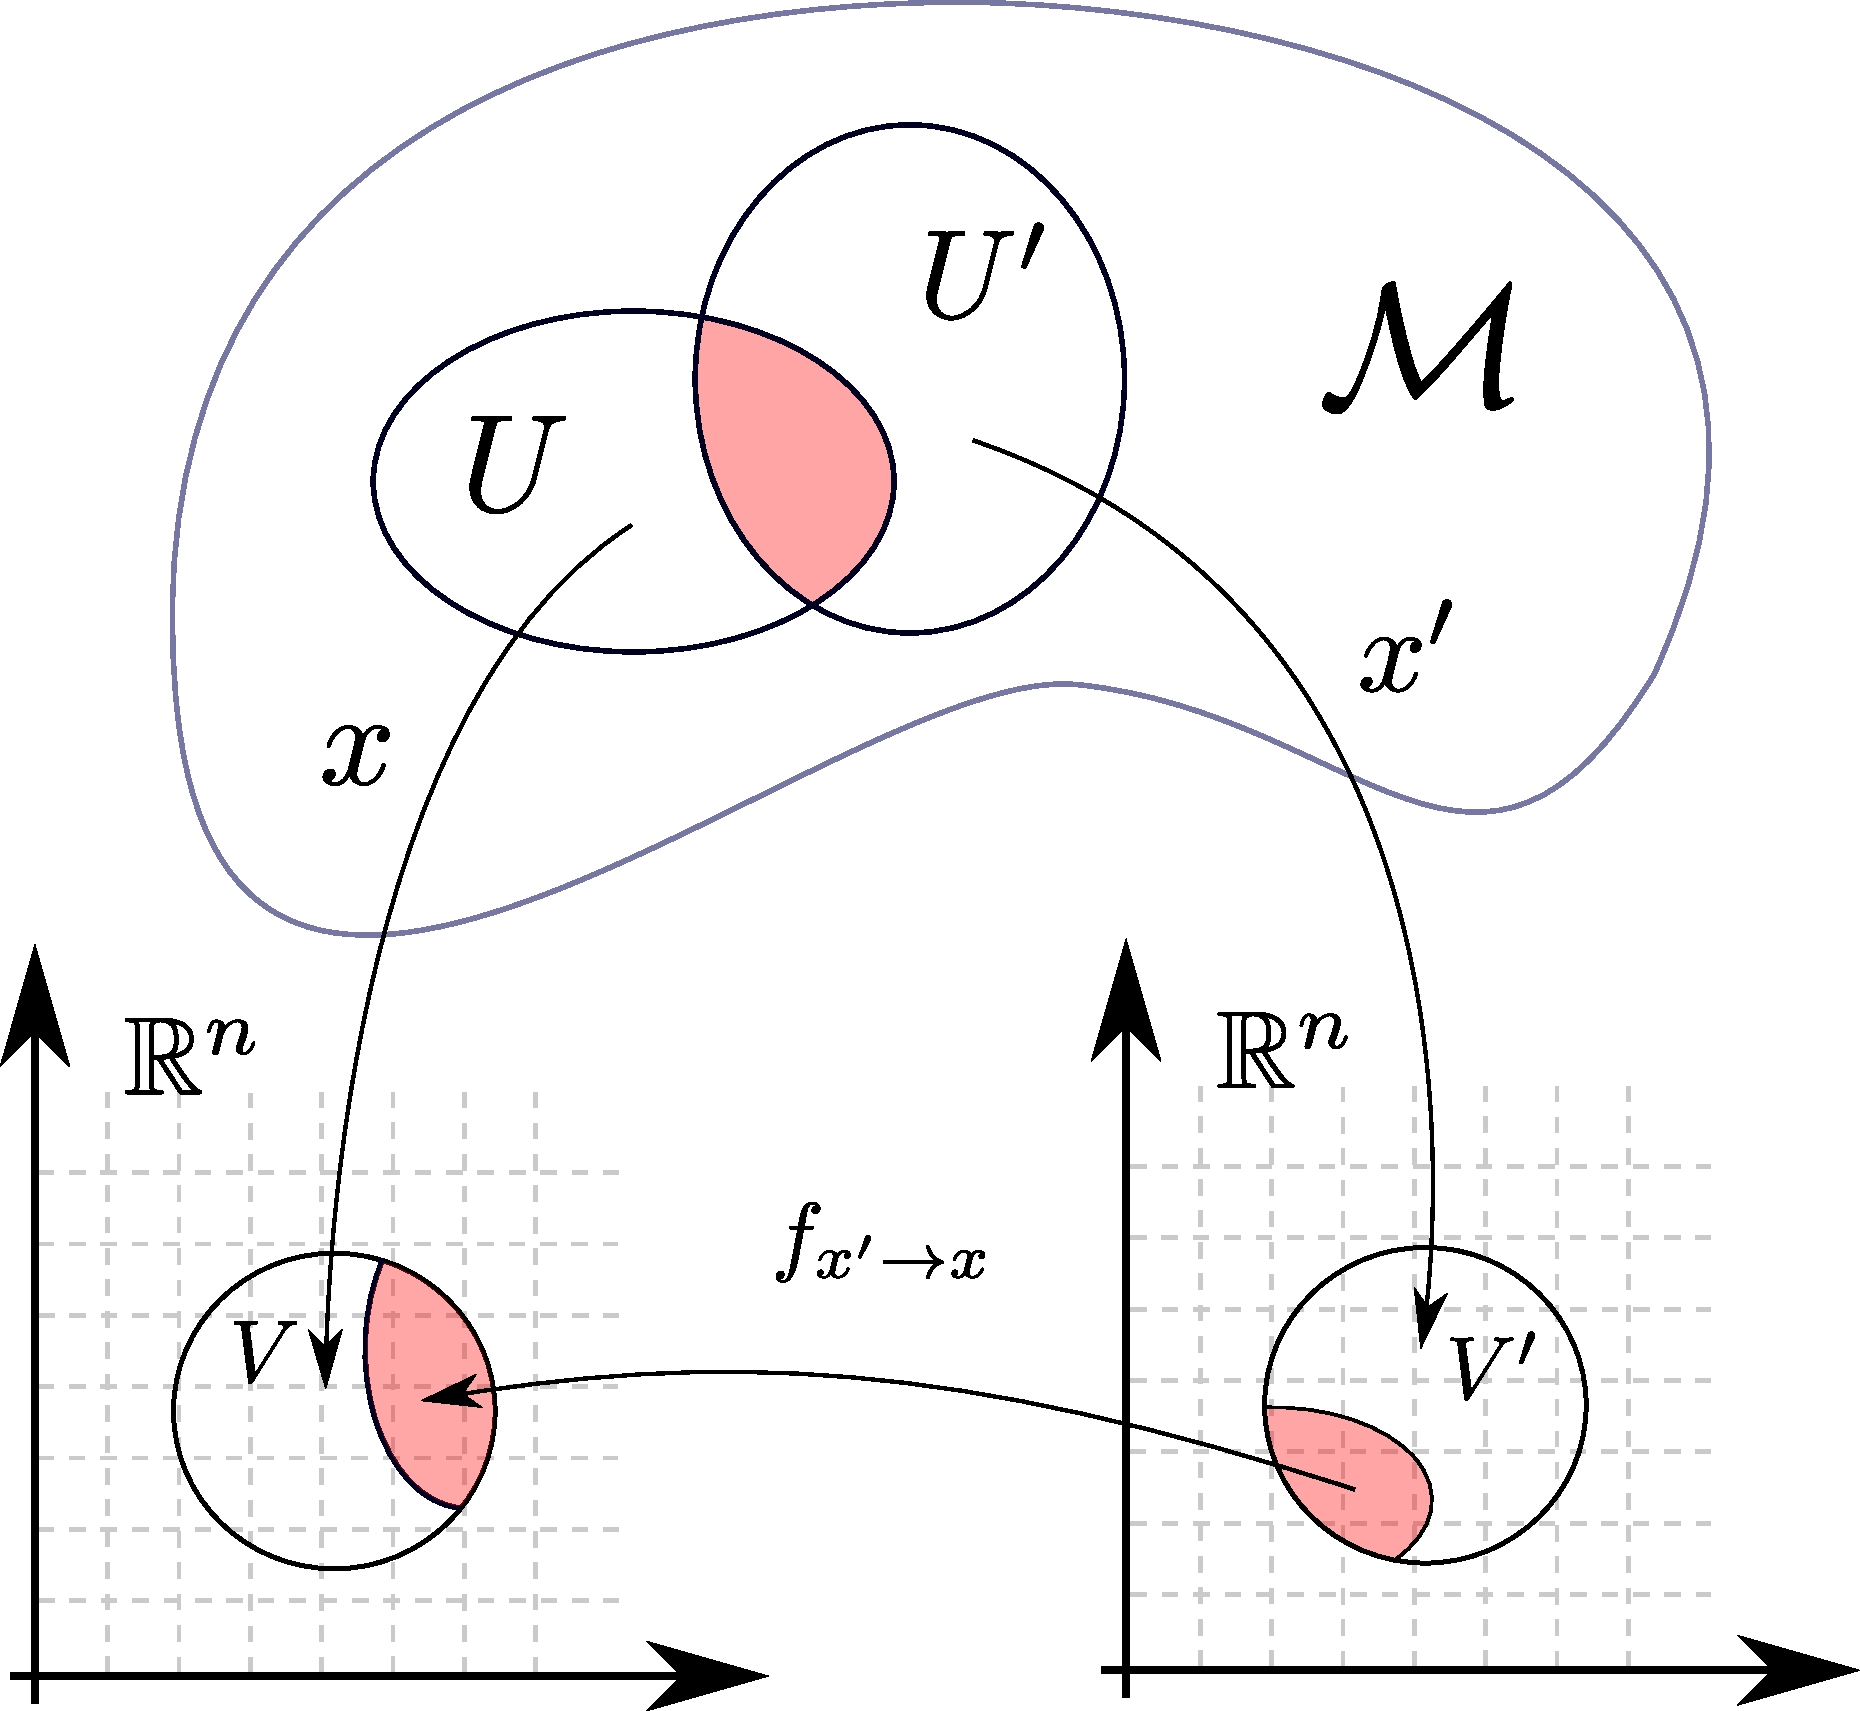
\includegraphics[width=0.6\textwidth]{figurer/transition_map.pdf}
    \caption{
        The transition map $f_{x'\rightarrow x}$ between two coordinate functions, $x$ and $x'$, maps between the images of these function, via the manifold $\Em$. 
        The function's domain and image are restricted to a (possibly empty) subset of the images of $x$ and $x'$. This is illustrated by the shaded regions in $V$ and $V'$. 
        }
    \label{fig: transition map}
\end{figure}

Consider two $m$- and $n$-dimensional smooth manifolds $\Em$ and $\mathcal N$.
Let $x$ denote the coordinates on $\Em$, while $y$ denotes the coordinates on $\mathcal N$.
We can define smooth functions between these manifolds similarly to how we define smooth coordinates.
Consider the function
%
\begin{equation}
    F: \Em \longmapsto \mathcal N.
\end{equation}
%
It is said to be smooth if, for all points $p \in\Em$, there is a set of local coordinates $x$ around $p$ and $y$ around $F(p)$ such that the map $\tilde F = y \circ F \circ x^{-1}$ is smooth.
This map may be illustrated by a diagram,
%
\begin{equation}
    % https://tikzcd.yichuanshen.de/#N4Igdg9gJgpgziAXAbVABwnAlgFyxMJZABgBoBGAXVJADcBDAGwFcYkQAdDgW3pwAsARoIAEAJQB63EAF9S6TLnyEUZYtTpNW7LrwEBjJiICys+SAzY8BIuVLqaDFm0SceffocYiAcmYVWyrYUGk7arroewuIShDIaMFAA5vBEoABmAE4Q0oh2IDgQSGQgjPSCMIwACorWKqUw6TggjlouIAAe-iBZOUj5hUgATK3O7OndvbkjBUWIAMyj4SAAnpPZuSWDC0vtSbKUMkA
\begin{tikzcd}
    \mathcal M \arrow[d, "x"] \arrow[r, "F"] & \mathcal N \arrow[d, "y"] \\
    \mathbb R^m \arrow[r, "\tilde F"]               & \mathbb R^n              
    \end{tikzcd}
    %
\end{equation}
%
%
We will not be careful with the distinction between $F$, the function between the abstract manifolds, and $\tilde F$, the function of their coordinates, but rather denote both by $F(x)$.
We may take the partial derivative of such a function with respect to the coordinates $x$, $\pdv{F}/{x^\mu}$.
However, this is dependent on our choice of coordinates, as a set of local coordinates can always be scaled arbitrarily.
Any physical theory must be independent of our choice of coordinates, so our next task is to define the properties of a smooth manifold in a coordinate-independent way.


\subsection{Vectors and tensors}

A curve $\gamma$ through $\Em$ is a function from $\R$ to $\Em$,
%
\begin{align}
    \gamma : \R &\longmapsto \Em \\
    \lambda & \longmapsto \gamma(\lambda).
\end{align}
%
Such curves are often denoted only by their coordinates and the parameter $\lambda$, $x^\mu(\lambda) = (x^\mu \circ \gamma)(\lambda)$.
With this curve, we can take the directional derivative of a real-valued function on the manifold, $f: \Em \mapsto \R$.
Assume $\gamma(\lambda = 0) = p$.
As we are always taking the derivative of functions between $\R^n$, for different $n$, we can use the chain rule.
The directional derivative of $f$ at $p$, given by this curve $\gamma$, is then
%
\begin{equation}
    \odv{}{\lambda} f(x(\lambda)) \bigg |_p = \odv{x^\mu}{\lambda} \bigg |_{\lambda = 0}  \pdv{}{x^\mu} f(x) \bigg |_p.
\end{equation}
%
The set of all such directional derivatives, $\odv{}/{\lambda}$ at $p$, form a vector space, $T_p \Em$, called the \emph{tangent space}.
The tangent space is illustrated in \autoref{fig: tangent space}.


\begin{figure}[H]
    \centering
    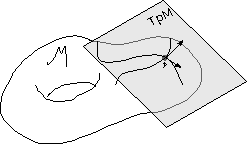
\includegraphics[width=0.7\textwidth]{figurer/tangent space.pdf} 
    \caption{
        The tangent space $T_p \Em$, the shaded rectangle, is the sett of all directional derivatives at $p\in \Em$. A directional derivative is defined in terms of a curve that passes through $p$.
        } 
    \label{fig: tangent space}
\end{figure} 


The coordinates $x^\mu$ induce a basis of this vector space, namely partial derivatives with respect to the coordinate functions at $p$,
%
\begin{equation}
    e_\mu = \pdv{}{x^\mu} \bigg|_p = \partial_\mu|_p, \quad \mu \in \{0, ... n-1\}.
\end{equation}
%
Any element $v \in T_p \Em$ can therefore be written
%
\begin{equation}
    v = v^\mu \partial_\mu |_p = \odv{x^\mu}{\lambda}\Big |_{\lambda = 0} \pdv{}{x^\mu}\Big |_p.
\end{equation}
%
Here, $\lambda$ is the parameter of the curve corresponding to the directional derivative $v$.\footnote{%
There is not only one curve corresponding to any directional derivative but rather an equivalence class. We will gloss over this technicality, as it does not affect our work.
}
The evaluation at $\lambda = 0$ and $p$ will often be implicit for ease of notation.
This directional derivative acts on functions $f : \Em \mapsto \R$ as
%
\begin{equation}
    v(f) = v^\mu \partial_\mu f.
\end{equation}
%




A map $F$ between two manifolds $\Em$ and $\mathcal N$ also induces a map between the tangent spaces of these manifolds.
This is the \emph{differential} of $F$ at $p$, 
%
\begin{align}
    \dd F_p: T_p \Em & \longmapsto T_p \mathcal N, \\
    v & \longmapsto \dd F_p (v). 
\end{align}
%
$\dd F_p(v)$ is an element of $T_p \mathcal N$, i.e., it is a directional derivative on $\mathcal N$.
It is defined by how it acts on functions $g: \mathcal N \mapsto \R$,
%
\begin{equation}
    \dd F_p(v) (g) = v(g \circ F),
\end{equation}
%
It thus acts on functions on $\mathcal N$ by ``extending'' the derivative $v$.
This is a linear map between vector spaces and may be written in component form by considering the differentials of the coordinate functions.
Denote the coordinates of $\mathcal N$ by $y^\mu$, and $y^\mu \circ F = F^\mu$.
Then,
%
\begin{equation}
    \dd F_p (\partial_\mu) (g) = \partial_\mu (g \circ F) |_p 
    = \pdv{F^\nu}{x^\mu}\Big |_p \pdv{g}{y^\nu} \Big  |_{F(p)},
\end{equation}
%
or more suggestively
%
\begin{equation}
    \dd F \left( \pdv{}{x^\mu} \right) = \pdv{F^\nu}{x^\mu} \pdv{}{y_\nu}.
\end{equation}
%
This is a linear map of vectors between two vectors by the matrix $A_\mu{}^\nu = \partial_\mu F^\nu$.
The differential is thus a generalization of the Jacobian.
In the case of a real valued function, $f: \Em \mapsto \R$, and $g : \R \mapsto \R$, we get
%
\begin{equation}
    \dd f (v) (g) 
    = v(g \circ f) 
    = (v^\mu \partial_\mu f) \, \odv{g}{y}.
\end{equation}
%
$\dd f$ is thus a map from $T_p \Em$ to $T_{f(p)}\R$, which is isomorphic to $\R$.
The $g$ be the identity function, so that $\odv{g}/{y} = 1$.
Then, the differential of a scalar function, also called a 1-form, is a map from vectors $v$ to real numbers,
%
\begin{equation}
    \label{covectors i.e. one forms}
    \dd f(v) := v^\mu \partial_\mu f.
\end{equation}
%
The set of all linear maps from a vector space $V$ to the real numbers is called the \emph{dual space} of $V$, denoted $V^*$.
This is a new vector space with the same dimensionality as $V$.
We denote the dual of $T_p \Em$ as $T_p^* \Em$.
We can regard each coordinate function as a real-valued function with a corresponding differential.
This differential obeys
%
\begin{equation}
    \dd x^\mu (\partial_\nu) = \pdv{x^\mu}{x_\nu} = \delta^\mu_\nu.
\end{equation}
%
The differentials of the coordinate functions thus form a basis for $T^*_p \Em$, called the dual basis.
Any differential $\dd f$ can thus be written as $\dd f = \omega_\mu \dd x^\nu$ for some components $\omega_\mu$.
We finde the components by applying the differential to the coordinate basis, $\dd f(\partial_\mu) = \partial_\mu f = \omega_\mu$.
In other words, we recover the classical expression 
%
\begin{equation}
    \dd f = \pdv{f}{x^\mu} \dd x^\mu,
\end{equation}
however we now interpret it as a covector-field instead of an ``infinitesimal displacement''.

Linear maps from vectors to real numbers is generalized by \emph{tensors}.
Given a vector space $V$, a general $(n, m)$ tensor $T$ is a multilinear map, which associates $n$ elements from $V$ and $m$ from its dual $V^*$ to the real numbers, i.e.,
%
\begin{align}
    T: V \times V \times \dots\times V^* \times \dots &\longmapsto \R, \\
    (v, u\dots; \omega, \dots) & \longmapsto T(v, u, \dots; \omega, \dots).
\end{align}
%
Multilinear means that $T$ is linear in each argument.
The set of all such maps is the tensor product space $V\otimes V \otimes \dots \otimes V^* \otimes \dots$, a $\dim(V)^{n+m}$-dimensional vector space.
If $\{e_\mu\}$ and $\{e^\mu\}$ are the basis for $V$ and $V^*$, then we can write the basis of this of the tensor product space as $ \{e_{\mu} \otimes \dots \otimes e^{\nu} \otimes \dots \}$.
The tensor can thus be written
%
\begin{equation}
    T =
     T^{\mu \nu\dots}{}_{\rho\dots} \, e_{\mu}\otimes e_\nu \otimes \dots e^\rho\otimes\dots, \quad
    T^{\mu \nu\dots}{}_{\rho\dots} = T(e^\mu, e^\nu, \dots; e_\rho, \dots).
\end{equation}
% 
We often what to decopose a tensor down into its symmetric and antisymmetric parts.
To do this, we introduce the symmetrization of a tensor $T$, 
%
\begin{equation}
    T_{(\mu_1\dots\mu_n)} 
    = \frac{1}{n!} \sum_{\sigma \in S_n} 
    T_{\mu_{\sigma(1)} \dots \mu_{\sigma(n)}},
\end{equation}
%
where $S_n$ is the set of all permutations of $n$ objects.
The antisymmetrization of a tensor is defined as
%
\begin{equation}
    T_{[\mu_1\dots\mu_n]} 
    = \frac{1}{n!} \sum_{\sigma \in S_n} \text{sgn}(\sigma)  
    T_{\mu_{\sigma(1)} \dots\mu_{\sigma(n)}}.
\end{equation}
%
The function $\text{\sigma} = \pm 1$, depending on if $\sigma$ is a even or odd permutation.
We may now write
%
\begin{equation}
    T_{\mu \nu} = T_{(\mu \nu)} + T_{[\mu \nu]}.
\end{equation}




\subsection{Geometry and the metric}
\label{subsection: goemetry and the metric}

The metric is a symmetric, non-degenerate $(0, 2)$ tensor
%
\begin{equation}
    \dd s^2 = g_{\mu \nu} \, \dd x^\mu \otimes \dd x^\nu.
\end{equation}
%
It defines the geometry of the manifold $\Em$ and is the main object of study in general relativity.
As it is invertible, we can define $g^{\mu \nu} = (g^{-1})_{\mu \nu}$, which is the components of a $(2, 0)$ tensor.
We use this to raise and lower indices, as is done with the Minkowski metric $\eta_{\mu \nu}$ in special relativity.

Up until now, we have only considered the tangent space $T_p \Em$ at a point $p$ and the corresponding tensor-product spaces.
We are, however, more interested in \emph{fields} of vectors, covectors, or tensors.
For each point $p \in \Em$, a tensor field $T$ ``picks out'' a tensor $T(p)$ from each tensor product space corresponding to the tangent space at $p$, $T_p \Em$.
We will use a vector field to illustrate.
This vector field can be written as
%
\begin{equation}
    v(p) = v^\mu(p) \partial_\mu |_p. 
\end{equation}
%
We will mostly be working with the components $v^\mu$, which are functions of $\Em$.
For ease of notation, we write the vector as a function of the coordinates $x$.
The vector field $v(x)$ is unchanged by a coordinate-transformation $x^\mu \rightarrow {x'}^\mu$; the coordinates are only a tool for our convenience.
However, with a new set of coordinates, we get a new set of basis vectors, $\partial'_\mu$:
%
\begin{equation}
    v = v^\mu \partial_\mu = v^\mu \pdv{x'^\nu}{x^\mu} \partial'_\nu
    = v'^\mu \partial_\mu',
\end{equation}
%
This gives us the transformation rules for the components of vectors,
%
\begin{equation}
    v'^\mu = \pdv{x'^\mu}{x^\nu} v^\nu.
\end{equation}
%
Tangent vectors are also called \emph{contravariant} vectors, as their components transform contra to basis vectors.
For covectors, it is
%
\begin{equation}
    \omega'_\mu = \omega_\nu \pdv{x^\nu}{x'^\mu},
\end{equation}
%
which is why covectors also are called \emph{covariant} vectors.

The gradient of a scalar function $f$, $\dd f = \partial_\mu f \dd x^\mu$, is a coordinate-independent derivative, as $\partial_\mu f$ follows the transformation law for covectors.
We define the covariant derivative, $\nabla$, as a map from $(n, m)$ tensor fields to $(n, m+1)$ tensor fields.
When considering a scalar as a $(0, 0)$ tensor, we see that this generalizes the scalar derivative.
The components of a covariant derivative, $\nabla_\rho T^{\mu_1\dots}{}_{\nu_1, \dots}$, must follow the tensor transformation law. 
However, this is not strong enough to uniquely define $\nabla$.
We further assume
%
\begin{itemize}
    \item Linearity: $\nabla (T + S) = \nabla T + \nabla S$.
    \item The product rule: $\nabla (T \otimes S) = (\nabla T)\otimes S + T \otimes (\nabla S)$.
    \item Reduces to partial derivative for scalars: $\nabla_\mu f = \partial_\mu f$.
    \item Kronecker delta gives zero: $\nabla_\mu \delta^\rho_\nu = 0$.
\end{itemize}
%
With this, we can, in general, write the covariant derivative for vectors and covectors as~\autocite{carrollSpacetimeGeometryIntroduction2019}
%
\begin{align}
    \label{covariant derivative diff geom}
    \nabla_\mu v^\nu &= \partial_\mu v^\nu + \Gamma^\mu_{\nu \rho} v^\rho, \\
    \label{covariant derivative diff geom covector}
    \nabla_\mu \omega_\nu &= \partial_\mu \omega_\nu - \Gamma^\rho_{\mu \nu} \omega_\rho.
\end{align}
%
$\Gamma^{\mu}_{\nu \rho}$ are called \emph{Christoffel symbols}.
The generalization for higher-order tensors is straightforward, 
%
\begin{equation}
    \nabla_\mu T^{\nu\dots}{}_{\rho\dots}
    =
    \partial_\mu T^{\nu\dots}{}_{\rho\dots}
    + \Gamma^\mu_{\nu \lambda} T^{\lambda\dots}{}_{\rho\dots} +\dots
    - \Gamma^\lambda_{\mu \rho} T^{\mu\dots}{}_{\lambda\dots} -\dots.
\end{equation} 
%
This is still not enough to uniquely determine the covariant derivative.
We will furthermore assume $\Gamma^{\lambda}_{\mu \nu} = \Gamma^{\lambda}_{\nu \mu}$ and $\nabla_\mu g_{\nu \rho} = 0$.
With these, we can find an explicit formula of the Christoffel symbols in terms of the metric,
%
\begin{equation}
    \label{christoffel symbols from metric}
    \Gamma^\rho_{\mu \nu} = \frac{1}{2} g^{\rho \sigma} (\partial_\mu g_{\nu \sigma} - \partial_\sigma g_{\mu \nu} + \partial_{\nu}g_{\sigma \mu}).
\end{equation}
%
With the notion of a covariant derivative, we may also generalize \emph{parallel transport} to curved spaces.
The notion of parallel transport of a vector in flat $\R^n$ is intuitive---given a line $x^\mu(\lambda)$, a vector $v^\mu$ at $x^\mu(\lambda_0)$ is parallel transported to $v'^\mu$ at $x^\mu(\lambda_1)$ if you carry it along the line without ``turning it''.
To make this more precise, a vector field $v^\mu$ is parallel transported along $x^\mu(\lambda)$ if $\odv{}{\lambda} v^\mu = \odv{x^\nu}{\lambda} \partial_\nu v^\mu$ = 0.
We generalize this to curved spaces by replacing the partial derivative with a covariant derivative, and so the criterion for parallel transport is
%
\begin{equation}
    \label{parallel transport criterion}
    \odv{x^\mu}{\lambda} \nabla_\mu v^\nu = 0.
\end{equation}
%
With this, we can imagine creating a special class of paths, called \emph{geodesics}, namely those which parallel transport their tangent vectors $\odv{x^\mu}{\lambda}$.
We imagine following an arrow we are holding without turning it as we walk.
Using the definition of parallel transport \autoref{parallel transport criterion}, together with the covariant derivative \autoref{covariant derivative diff geom}, we get the geodesic equation,
%
\begin{equation}
    \label{goedesic equation}
    \odv[2]{x^\mu}{\lambda} 
    + \Gamma^\mu_{\rho \sigma} \odv{x^\rho}{\lambda} \odv{x^\sigma}{\lambda}
    = 0.
\end{equation}
In a flat space, where the Christoffel symbols vanish, this reduces to the familiar criterion for straight lines, $\odv[2]{x^\mu}{\lambda} = 0$.

The curvature of a manifold $\Em$, with the metric $g_{\mu \nu}$, is encoded in the Riemann tensor.
It is defined by
%
\begin{equation}
    \label{Riemann tensor}
    [\nabla_\mu, \nabla_\nu] v^\rho = R^{\rho}{}_{\sigma \mu \nu} v^\sigma,
\end{equation}
%
which in our case gives the explicit formula
%
\begin{equation}
    \label{riemann tensor in terms of christoffel symbols}
    R^\rho{}_{\sigma \mu \nu} 
    = \partial_{\mu} \Gamma^{\rho}_{\nu \sigma}
    - \partial_{\nu} \Gamma^{\rho}_{\mu \sigma}
    + \Gamma^{\rho}_{\mu \lambda} \Gamma^{\lambda}_{\nu \sigma}  
    - \Gamma^{\rho}_{\nu \lambda} \Gamma^{\lambda}_{\mu \sigma}.
\end{equation}
%
This form gives us several useful identities, such as
%
\begin{equation}
    R_{\rho \sigma \mu \nu} 
    = 
    R_{[\rho \sigma] \mu \nu}
    =
    R_{\rho \sigma [\mu \nu]}
    =
    R_{\mu \nu \rho \sigma }.
\end{equation}
%
Using the Jacobi identity of the commutator, we have
%
\begin{equation}
    \label{Jacobi identity differential geometry}
    [\nabla_\mu, [\nabla_\nu, \nabla_\sigma]]
    + [\nabla_\sigma, [\nabla_\mu, \nabla_\nu]]
    + [\nabla_\nu, [\nabla_\sigma, \nabla_\mu]] = 0.
\end{equation}
%
If we apply this on $\delta^{\mu}_{\nu}$, we get the differential Bianchi identity, compactly written
%
\begin{equation}
    \label{Binachi identiy}
    \nabla_{[\mu}R_{\nu \rho]\sigma \eta} = 0.
\end{equation}
%
Although the Christoffel symbols are not tensors, the Riemann tensor is due to its definition using covariant derivatives.
We can therefore contract some of its indices to get other tensor quantities.
We define the Ricci tensor and Ricci scalar as
%
\begin{align}
    \label{Ricci tensor}
    R_{\mu \nu} &= R^{\rho}{}_{\mu \rho \nu}, \\
    \label{Ricci scalar}
    R &= R^{\mu}{}_{\mu} = g^{\mu \nu} R_{\mu \nu}.
\end{align}


To interpret the Riemann tensor, we define the parallel propagator $P$.
A vector that is parallel transported along a curve parametrized by $\lambda$ should then obey
%
\begin{equation}
    v^\mu(\lambda) = P^\mu{}_\nu(\lambda) v^\nu.
\end{equation}
%
Inserting this into the equation for parallel transport, \autoref{parallel transport criterion}, this operator must obey
%
\begin{equation}
    \odv{}{\lambda} P^\mu{}_\nu = - \Gamma^\mu_{\rho \sigma}  \odv{x^\rho}{\lambda}P^\sigma{}_\nu.
\end{equation}
%
This has the same form as the definition of the unitary time-evolution operator in quantum mechanics, and we could therefore write down a solution involving an exponential and a path ordering operator, $\mathcal P$, analogous to the time ordering operator from quantum mechanics.
We may rewrite the equation as an integral equation,
%
\begin{equation}
    P^\mu{}_\nu(\lambda) = \delta^\mu_\nu 
    - \int^\lambda_0 \dd \lambda' \Gamma^\mu_{\rho \sigma} V^\rho P^\sigma{}_\nu,
\end{equation}
%
where we denote $\odv{x^\mu}{\lambda} = V^\mu$.
This allows us to solve the equation iteratively.
If $\lambda \leq \epsilon \ll 1$, we expect this to converge as long as the $g$ is well-behaved.
Starting with the zeroth-order solution $P^{\mu}{}_\nu = \delta^\mu_\nu$ and iterating twice gives us
%
\begin{equation}
    \label{iterative paralell propagator}
    P^\mu{}_\nu(\lambda) 
    = 
    \delta^\mu_\nu 
    - \int_0^\lambda \dd \lambda' \, 
    \Gamma^\mu_{\rho \nu} V^\rho
    + \int_0^{\lambda} \dd \lambda ' \int_0^{\lambda'} \dd \lambda ''\,
    \Gamma^\mu_{\rho \sigma} \Gamma^\sigma_{\eta \nu} V^\rho V^\eta
    + \Oh(\epsilon^3).
\end{equation}
%
With this, we will investigate how much a vector $v^\mu$ is changed by being parallel transported around in a small loop, as illustrated in \autoref{fig: parallel transport in loop}.

\begin{figure}[H]
    \centering
    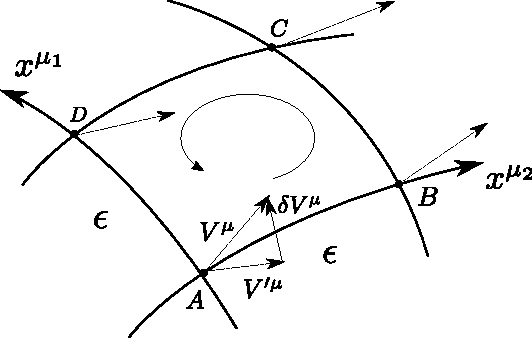
\includegraphics[width=0.6\textwidth]{figurer/parallel_transport.pdf}
    \caption{A vector $v^\mu$ is parallel transported in a small, closed loop, defined by the coordinate functions $x^{\mu_1}$ and $x^{\mu_2}$.
    As a consequence of the curvature, it has changed by $\delta v^\mu$ by the time it arrives back at $A$.}
    \label{fig: parallel transport in loop}
\end{figure}


We transport $v^\mu$ along the coordinate lines.
These are lines where either of the coordinate functions $x^{\mu_1}$ or $x^{\mu_2}$ are equal to $0$ or $\epsilon$.
Here, the indices $\mu_1$ and $\mu_2$ are not free but identify the two coordinate functions which define this loop.
The line from $A$ to $B$, defined by $x^{\mu_1} = 0$, is parametrized by $x^\mu(\lambda) = \lambda \delta^\mu_{\mu_2}$, so $ V^\mu = \delta^\mu_{\mu_2} $.
The Christoffel symbol along this line is
%
\begin{equation}
    \Gamma^{\mu}_{\nu \rho}(\lambda) 
    = \Gamma^{\mu}_{\nu \rho}|_A
    + \lambda \partial_{\mu_2} \Gamma^{\mu}_{\nu \rho}|_A + \Oh(\epsilon^2).
\end{equation}
%
Inserting this into \autoref{iterative paralell propagator}, we get
%
\begin{equation}
    P^\mu{}_\nu(\epsilon)
    = \delta^\mu_\nu 
    - \epsilon \Gamma^{\mu}_{\nu \mu_2}|_A
    + \frac{1}{2} \epsilon^2 
    \left(
        \Gamma^\mu_{\mu_2 \sigma}\Gamma^\sigma_{\mu_2 \nu} |_A 
        -\partial_{\mu_2} \Gamma^{\mu}_{\nu \mu_2}|_A 
    \right)
    + \Oh(\epsilon^3).
\end{equation}
%
Next, from $B$ to $C$, the line is $x^\mu(\lambda) = \epsilon \delta^\mu_{\mu_2} + \lambda \delta^{\mu}_{\mu_1}$, so $V^\mu = \delta^\mu_{\mu_1}$, and the Christoffel symbols are 
$ 
\Gamma^{\mu}_{\nu\rho}
= 
\Gamma^{\mu}_{\nu \rho}|_B
+ \lambda \partial_{\mu_1} \Gamma^{\mu}_{\nu \rho}|_B
$
to fist order in $\lambda$.
Here, we have to expand once more to evaluate the symbols at $A$.
Then, we get
%
\begin{equation}
    \Gamma^{\mu}_{\nu\rho}
    =
    \Gamma^{\mu}_{\nu \rho}|_A + \epsilon \partial_{\mu_2} \Gamma^{\mu}_{\nu \rho}|_A
    + \lambda \partial_{\mu_1} \Gamma^{\mu}_{\nu \rho}|_A + \Oh(\epsilon^2),
\end{equation}
%
The parallel propagator from $B$ to $C$ is then
%
\begin{equation}
    P^{\mu}{}_\nu(\epsilon)
    = 
    \delta^\mu_\nu
    - \epsilon \Gamma^{\mu}_{\nu \mu_1}|_A 
    + \frac{1}{2}\epsilon^2
    \left(
        \Gamma^\mu_{\sigma \mu_1}\Gamma^\sigma_{\nu \mu_1}|_A
        - \partial_{\mu_1} \Gamma^{\mu}_{\nu \mu_1}|_A
        - 2 \partial_{\mu_2} \Gamma^{\mu}_{\nu \mu_1}|_A
    \right)
    + \Oh(\epsilon^3),
\end{equation}
%
Which gives the combined propagator from $A$ to $C$, to and including second order in $\epsilon$, as
%
\begin{align}
    \nonumber
    {P_{AC}}^\mu{}_{\nu}
    & = 
    \left[ 
        \delta^\mu_\sigma 
        -\epsilon \Gamma^{\mu}_{\sigma \mu_1}
        + \frac{1}{2} \epsilon^2 
        \left(
        \Gamma^\mu_{\eta \mu_1}\Gamma^\eta_{\sigma \mu_1}
        - \partial_{\mu_2} \Gamma^{\mu}_{\sigma \mu_2}
        - 2 \partial_{\mu_2} \Gamma^{\mu}_{\sigma \mu_1}
        \right)
    \right]
    \cdot 
    \left[
        \delta^\sigma_\nu
        - \epsilon \Gamma^{\sigma}_{\nu \mu_2}
        + \frac{1}{2} \epsilon^2 
        \left(
            \Gamma^\sigma_{\eta \mu_2}\Gamma^\eta_{\nu \mu_2}
            - \partial_{\mu_2} \Gamma^{\sigma}_{\nu \mu_2}
        \right)
    \right] \\ \nonumber
    & =
    \delta^\mu_\nu
    - \epsilon 
    \left(
        \Gamma^{\mu}_{\nu \mu_1}
        +
        \Gamma^{\mu}_{\nu \mu_2}
    \right)
    + \epsilon^2
    \frac{1}{2}
    \left(  
        2\Gamma^{\mu}_{\sigma \mu_1} \Gamma^{\sigma}_{\nu \mu_2}
        + \Gamma^\mu_{\sigma \mu_1}\Gamma^\sigma_{\nu \mu_1}
        + \Gamma^\mu_{\sigma \mu_2}\Gamma^\sigma_{\nu \mu_2}
        - 2 \partial_{\mu_2} \Gamma^{\mu}_{\nu \mu_1}
        - \partial_{\mu_1} \Gamma^{\mu}_{\nu \mu_1}
        - \partial_{\mu_2} \Gamma^{\mu}_{\nu \mu_2}
    \right).
\end{align}
%
The parallel propagator for $CDA$ is the propagator for $ADC$ with its signs flipped. 
The $ADC$ propagator is the same as $ABC$, only with the $\mu_1$ and $\mu_2$ indices switched.
It is thus
%
\begin{align}
    \nonumber
    {P_{CA}}^\mu{}_\nu
    & =
    \delta^\mu_\nu
    + \epsilon 
    \left(
        \Gamma^{\mu}_{\nu \mu_2}
        +
        \Gamma^{\mu}_{\nu \mu_1}
    \right)
    + \epsilon^2
    \frac{1}{2}
    \left(  
        2\Gamma^{\mu}_{\sigma \mu_2} \Gamma^{\sigma}_{\nu \mu_1}
        + \Gamma^\mu_{\sigma \mu_2}\Gamma^\sigma_{\nu \mu_2}
        + \Gamma^\mu_{\sigma \mu_1}\Gamma^\sigma_{\nu \mu_1}
        + 2 \partial_{\mu_1} \Gamma^{\mu}_{\nu \mu_2}
        + \partial_{\mu_2} \Gamma^{\mu}_{\nu \mu_2}
        + \partial_{\mu_1} \Gamma^{\mu}_{\nu \mu_1}
    \right).
\end{align}
%
The full propagator, from $A$ to $A$, is $P^\mu{}_\nu = {P_{CA}}^\mu{}_\rho {P_{AC}}^\rho{}_\nu$.
The terms linear in $\epsilon$ vanish, and the same with the terms with two equal $\mu_i$-indices.
The change in the vector as it is rotated around the loop is therefore, to second order in $\epsilon$,
%
\begin{align}
    \delta v^\mu 
    = P^\mu{}_\nu v^\nu - v^\mu 
    = \epsilon^2  
    \left(
        \Gamma^\mu_{\sigma \mu_1} \Gamma^\sigma_{\nu \mu_2}
        -\Gamma^\mu_{\sigma \mu_2} \Gamma^\sigma_{\nu \mu_1}
        + \partial_{\mu_1} \Gamma^{\mu}_{\nu \mu_2}
        - \partial_{\mu_2} \Gamma^{\mu}_{\nu \mu_1} 
    \right) v^\nu.
\end{align}
Comparing with \autoref{riemann tensor in terms of christoffel symbols}, we see that this is the Riemann curvature tensor.
In other words, the Riemann tensor encodes how a vector is transformed when parallel transported in a small, closed loop.



\subsection{Integration on manifolds}
\label{subsection: integration on manifolds}

The integral of a scalar function on a manifold is not a coordinate-independent notion.
To obtain this, we must introduce $n$-forms.
A $n$-form $\omega$ is an antisymmetric $(0, n)$ tensor.
This means that it has coordinates which obey $\omega_{\mu_1 \dots \mu_n} = \omega_{[\mu_1 \dots \mu_n]}$.
The $n$-forms are ubiquitous objects in mathematics and physics, one example is the electromagnetic field-strength tensor $F_{\mu \nu}$, and they allow for the definition of coordinate independent integration and derivation.
The wedge product, $\wedge$ is a product that maps two $n$- and $m$-forms to an $n+m$-form, and is defined as
%
\begin{equation}
    (A\wedge B)_{\mu_1\dots\mu_{n+m}} = \frac{(n + m)!}{n! m!} A_{[\mu_1\dots\mu_n}B_{\mu_{n+1}\dots\mu_{n+m}]}.
\end{equation}
%
Furthermore, we define the exterior derivative, a map from $n$-forms to $n+1$-forms, defined by
%
\begin{equation}
    (\dd T)_{\mu_1 \dots \mu_{n+1}} = (n+1) \partial_{[\mu_1} T_{\mu_2\dots\mu_{n+1}]}.
\end{equation}
%
We are interested in a coordinated independent quantity that we can integrate over.
To that end, we define
%
\begin{equation}
    \dd^n x := \dd x^0 \wedge \dots \wedge \dd x^{n-1}
    = \frac{1}{n!} \varepsilon_{\mu_1 \dots \mu_n}  
    \dd x^{\mu_1} \wedge \dots \wedge \dd x^{\mu_n},
\end{equation}
%
Where $\varepsilon_{\mu_1 \dots \mu_n}$ is the Levi-Civita symbol.
Given a different set of coordinates, $x'^\mu$, these are related by
%
\begin{equation}
    \dd^n x = \det\left( \pdv{x}{x'} \right) \, \dd^n x',
\end{equation}
%
where we have used the relation $\varepsilon_{\mu_1 \dots \mu_n}  \det(A) = \varepsilon_{\nu_1 \dots \nu_n} A^{\nu_1}{}_{\mu_1} \dots A^{\nu_n}{}_{\mu_n}$.  
We define $|g| = |\det(g_{\mu \nu })|$, which, by the transformation properties of tensors, transforms as
%
\begin{equation}
    \sqrt{|g'|} = \left| \det\left(\pdv{x'}{x} \right) \right| \sqrt{|g'|},
\end{equation}
%
This means we can use $|g|$ to compensate for the transformation of $\dd^n x$, and get a volume form with a coordinate independent definition,
%
\begin{equation}
    \dd V = \sqrt{|g|} \, \dd^n x = \sqrt{|g'|} \, \dd^n x'.
\end{equation}
%
With this, we can integrate scalars in a well-defined way by mapping them to a corresponding $n$-form, $f \rightarrow f \dd V$.
We define the integral of a scalar function $f$ on a manifold $\Em$ with a metric $g$ as
%
\begin{equation}
    I = \int_\Em \dd V \, f =  \int_{\Em} \dd^n x \, \sqrt{|g(x)|} \, f(x).  
\end{equation}


Stoke's theorem generalizes the fundamental theorem of calculus and the divergence theorem to manifolds.
Let $\Em$ be a differential manifold of dimension $n$, with the boundary $\partial \Em$.
Stoke's theorem says that, for an $n-1$-form $\omega$,
%
\begin{equation}
    \int_\Em \dd \omega = \int_{\partial \Em}  \omega. 
\end{equation}

Stoke's theorem then implies a generalized divergence theorem.
The boundary of $\Em$ is a $n-1$ manifold dimensional, and a metric $g$ on $\Em$ will induce a new metric $\gamma$ on $\partial \Em$.
This metric corresponds to the restriction of $g$ to $\partial \Em$.
Furthermore, there will be a vector field $n^\mu$ of normalized vectors orthogonal to all elements of $T \partial \Em$.
This theorem states that for a vector field $V^\mu$ on $\Em$,
%
\begin{equation}
    \label{generalized divergence theorem}
    \int_\Em \dd^n x \, \sqrt{|g|} \,  \nabla_\mu V^\mu 
    = \int_{\partial \Em} \dd^{n-1}y \, \sqrt{|\gamma|} \, n_\mu V^\mu.
\end{equation}
